\pagenumbering{arabic}%DO NOT REMOVE THIS
\chapter{Introduction}\label{ch:intro}
Reductive evolution is the process of the genome of an organism shrinking over time, with respect to both the number of base pairs and genes. Some species of bacteria have experienced reductive evolution over the course of millions of years, and this reduction in their genome has lead to a loss of genes, certain regulatory abilities, etc. For example, some strains of the marine cyanobacteria \textit{Prochlorococcus} have experienced a reduction of nearly 40\% of their base pairs when compared to larger strains of their closest living relative, \textit{Synechococcus}\cite{sun_zhiyi_blanchard}. Despite being extensively studied, the mechanisms and full impact of reductive evolution are not fully understood and are an area of ongoing research. 

Although it would provide more conclusive evidence, performing \textit{in vivo} experiments is often impractical because of the difficulty or impossibility of reproducing natural environmental conditions in a lab. Such experiments are often too costly in terms of both time and resources. As an alternative, \textit{in silico experimental evolution} is one option that can be used to study the conditions under which an organism's genome may become reduced. In this method, organisms and their evolution over thousands or millions of generations are simulated in software. In this manner, one can control and evaluate every aspect of their evolution over time and a full record of their lineage may be maintained and studied, allowing one to go back and closely examine every step of the evolutionary period for a greater understanding of the factors that lead to specific effects on the genome. The in silico tool \textit{Aevol} is one such platform which realistically models bacterial genomes and evolution, allowing one to draw conclusions about their real-world counterparts. In the following thesis, we present the results of our experiments in artificial evolution which aim to identify and evaluate several factors which potentially lead to changes in genome structure and a reduced genome in simulated bacteria using the Aevol platform. 

\section{Problem Statement} \label{problem_statement}
Among the difficulties of studying reductive evolution with in vivo evolutionary experiments, one of the most difficult obstacles to overcome is the lack of a full ancestral record. This lack of a full phylogeny can make it difficult or impossible to tell exactly when and how a specific event occurred, or a trait evolved or was lost, as illustrated in Figure \ref{fig:phylogeny03} below. 
\begin{figure}[h]
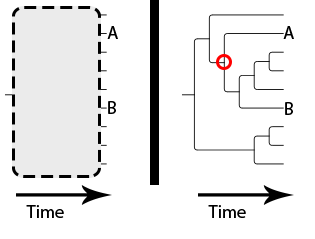
\includegraphics[scale=0.75]{phylogeny03}
\centering
\caption[Unknown phylogeny]{An illustration of unknown phylogeny. Since the phylogenetic information under the shaded box is typically not known, the point of divergence (red circle) can't be determined.}
\label{fig:phylogeny03}
\end{figure}
In this example, we are comparing two related organisms A and B and we are trying to determine when and how a specific trait was gained or lost by one of the organisms. This may be useful, for example, if we are attempting to estimate the relative importance (due to conservation over many generations) of some trait. Without the phylogenetic information (under the shaded box) we may not be able to identify the point in their evolutionary history at which the two organisms diverged, making time estimates difficult or impossible.

Another major downside to \textit{in vivo} evolutionary experiments is that they are slow. For example, the well-known E. coli Long-Term Evolution Experiment (LTEE) by Profesor Lenski at Michigan State University has been ongoing since February of 1988 and only passed generation 65,000 in 2016, 28 years later. 

As an alternative to in vivo experiments, \textit{in silico} evolutionary experiments are well-suited to the task of studying reductive evolution. Generations of organisms may be evolved within a very short time period, and a full "fossil record" of each lineage may be kept on disk for further analysis. 

The in silico tool Aevol has a realistic artificial chemistry model which was developed specifically to study genome structure. It contains tools to analyze the robustness, fitness, and evolvability of digital organisms over time.  

\section{Report outline}
This chapter serves as the introduction to the thesis and the research problem we are facing. In Chapter~\ref{ch:background}, we provide some necessary background information on reductive evolution, in silico evolution in general, and Aevol in particular. Chapter~\ref{ch:methods} describes our experimental setup. Chapter~\ref{ch:results_discussion}
provides the results and analysis of our experiments, and Chapter~\ref{ch:conclusion} presents our conclusions. 


